% 宇宙的演化
%% 还需要插入预备知识等等

宇宙演化可以大约分为两个时期,(详细可见\autoref{UniEvo_tab1}),从创世之初($t=0$) 到创世后3分钟我们可以称为前物质时期.这个时期可以大致分为两个时期:从宇宙诞生后到$10^{-43}$秒,此时宇宙沐浴于$10^{18}$GeV的高温中,四大相互作用被统一在一起.随后到$10^{-34}$秒宇宙在高温中经历\textbf{暴涨}(Inflation),宇宙尺度因子迅速扩大(详见\autoref{UniEvo_fig1}).在暴涨快结束时超对称破缺,宇宙中的重元素开始产生.

\begin{table}[ht]
\centering
\caption{宇宙大事记(问号表示不确定)}\label{UniEvo_tab1}
\begin{tabular}{|r|r|r|}
\hline
 & 时间 & 能量 \\
\hline
普朗克时间奇点? & $<10^{-43}$s & $10^{18}$GeV \\
\hline
弦论尺度?       & $>10^{-43}$s & $<10^{18}$ GeV \\
\hline
超统一?         & $\sim 10^{-36}$s & $10^{15}$GeV \\
\hline
暴涨开始?       & $>10^{-34}$s & $<10^{15} $GeV \\
\hline
超对称破缺?     & $<10^{-10}$s & $>1$ TeV \\
\hline
重元素产生?     & $<10^{-10}$s & $>1$ TeV \\
\hline
电弱统一时期    & $10^{-10}$s & 1 TeV \\
\hline
夸克-强子转换时期 & $10^{-4}$s & $10^2$ MeV \\
\hline
核子冷却        & 0.01s & 10 MeV \\
\hline
中微子退偶      & 1 s  & 1 MeV \\
\hline
大爆炸原核初合成  & 3 min & 0.1 MeV \\
\hline
物质-辐射密度相等 & $10^4$ yrs  & 1 eV \\
\hline
再融合 & $10^5$ yrs  & 0.1 eV \\
\hline
宇宙黑暗时期 & $10^5 - 10^8$ yrs  &  \\
\hline
再电离 & $10^8$ yrs  &  \\
\hline
星系形成 & $\sim 6 \times 10^8$ yrs  &  \\
\hline
暗能量 & $\sim 10^9$  yrs  &  \\
\hline
太阳系形成 & $ \sim 8 \times 10^9  $ yrs  &  \\
\hline
\end{tabular}
\end{table}

\begin{figure}[ht]
\centering
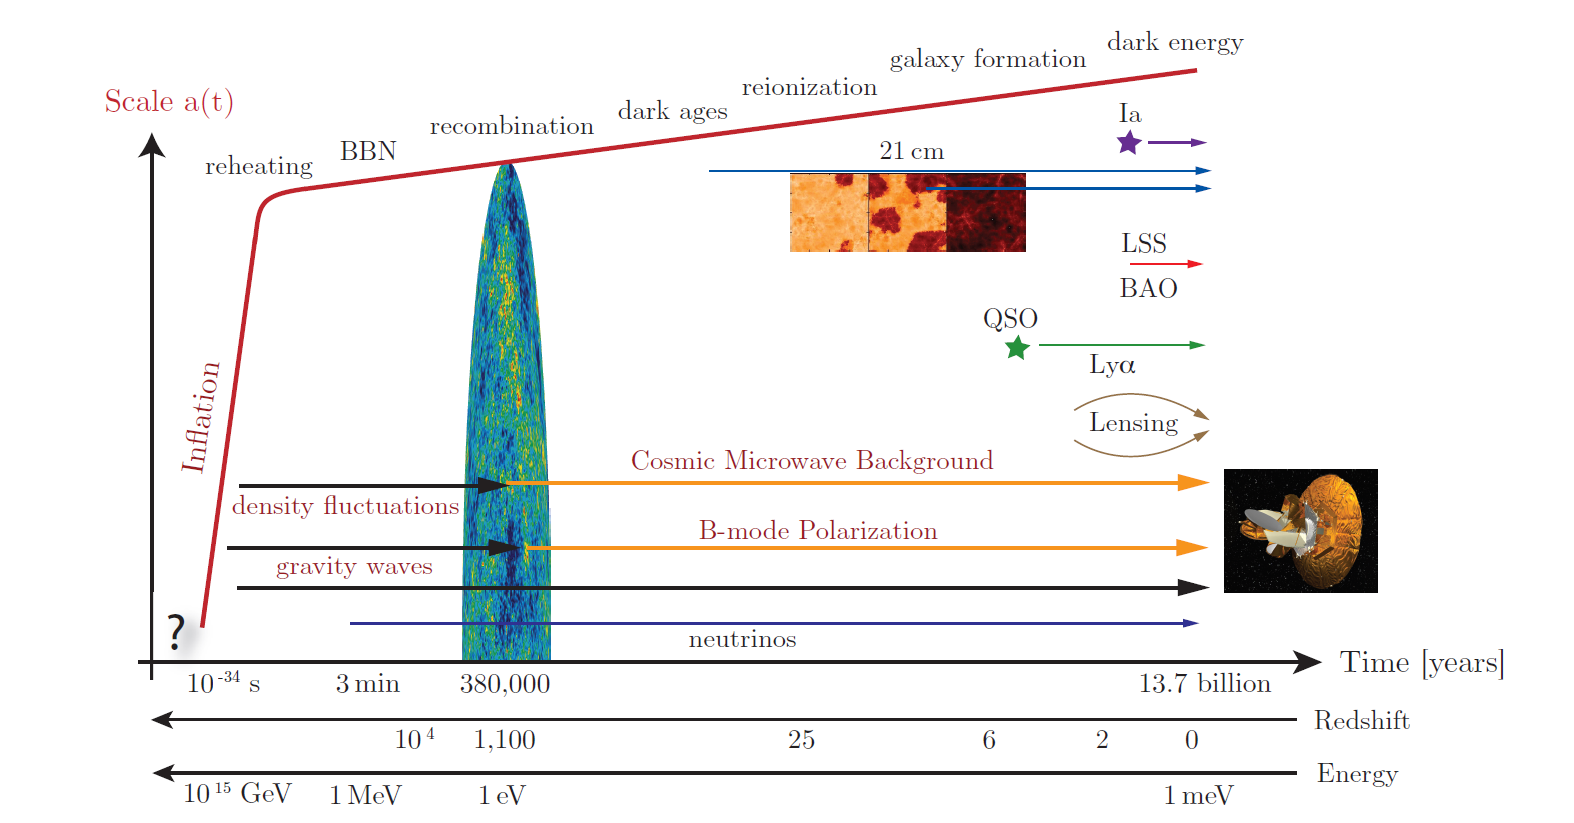
\includegraphics[width=30cm]{./figures/UniEvo_2.png}
\caption{宇宙尺度及成分表} \label{UniEvo_fig1}
\end{figure}

从$10^{-10}$ 秒到宇宙诞生后3分钟,宇宙暴涨结束,宇宙从$1$ TeV 迅速逐渐冷却到 $0.1 $ MeV.在此期间暴涨所释放的能量把宇宙重新加热,宇宙中的电弱相互作用开始分离,夸克结合成强子,中子冷却下来,宇宙中的核子开始在相互作用下结合并形成,称为\textbf{原核初合成}(BBN);中微子在创世后1秒与其他核子退耦并此后不再与其他物质产生相互作用,一直传播到现在.此时,宇宙开始以辐射为主导,我们也称为辐射主导时期的开始,此外,宇宙中的原初扰动和引力波开始形成.

\begin{figure}[ht]
\centering
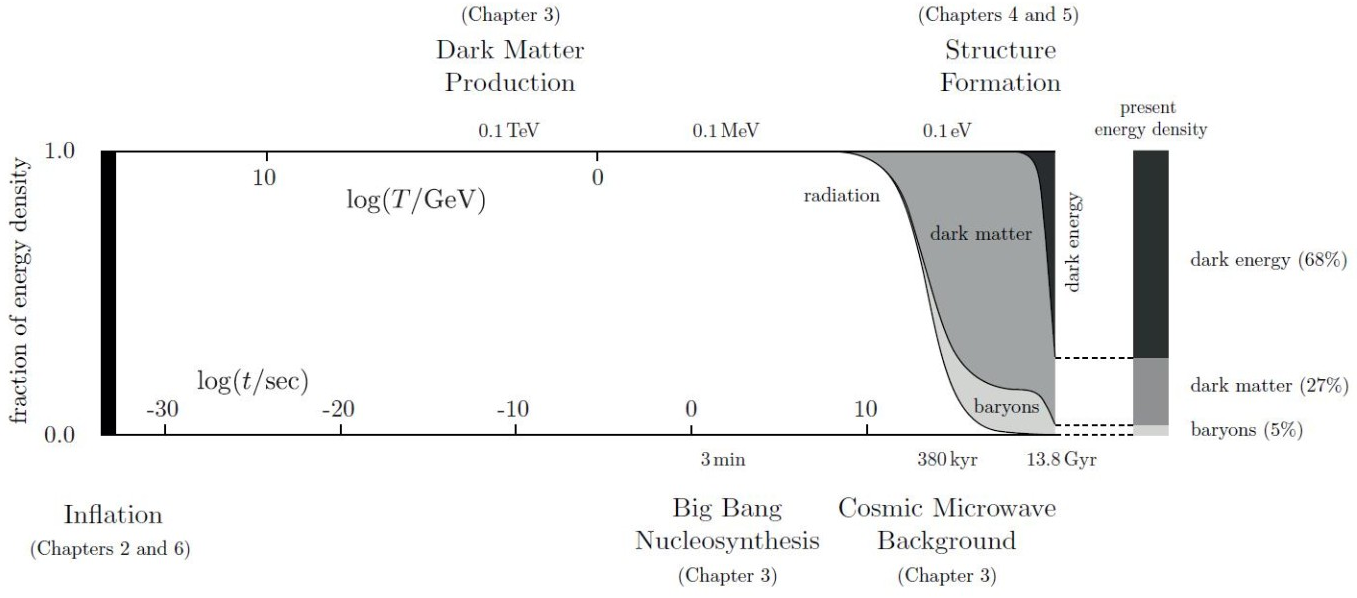
\includegraphics[width=30cm]{./figures/UniEvo_1.png}
\caption{宇宙成分变化} \label{UniEvo_fig2}
\end{figure}

从创世后3分钟到现在,我们可以称为后物质时期.我们也可以把这个时期大致地分为两个时期:从宇宙诞生后3分钟到380.000年,宇宙一直以辐射为主导(宇宙成分具体的演化可见\autoref{UniEvo_fig2}).随着宇宙的膨胀光子和物质从密度对等逐渐分离,且光子、物质和原初引力波进行充分的相互作用称为\textbf{再融合}(recombination),光子逐渐冷却下来形成\textbf{宇宙辐射背景}(CMB),期间暗物质开始形成.

从宇宙诞生后380.000年到现在,宇宙进入物质主导时期,另一部分光子形成了宇宙辐射背景并随着时间演化到现在,一部分光子和原初引力波相互作用后成为B-模极化光子; 一部分原初引力波和中微子并不参与到相互作用中,并随着时间演化直到现在.在此期间,各大星系形成于创世后$10^8$ 年之后,太阳系形成于$8\times 10^9$年.




